% !TeX root = ../thesis.tex
\chapter{Results}

\section{Data quality and completeness}

\section{The adaptive system in practice}
The adaptive difficulty system described in Section~\ref{sec:adaptivity} was used in two of the four experimental conditions (C and D). The non-adaptive conditions (A and B) presented exercises drawn from a balanced mix of all three difficulty levels in a semi-random order. This section examines how the adaptive system behaved in practice using both quantitative data and qualitative observations.\\ \\

\subsection{Elo trajectories}
Figure~\ref{fig:elo-trajectories} shows the Elo trajectories of five randomly selected participants from the adaptive conditions over the course of their 216 exercises. All five children started at the initial rating of 450, but their paths diverge quickly. The strongest participant (blue) climbed rapidly and reached the ceiling of 1000 within the first 50 exercises, remaining there for the rest of the study. Two others (green and orange) followed a slower upward trend, stabilising in the 800--950 range by the end of the training period. The remaining two (red and purple) settled in the 600--800 range, with visible fluctuations that reflect the system adjusting to their performance on individual exercises.\\ \\
Two things are worth noting. First, the trajectories are not smooth curves but jagged paths with frequent ups and downs. This is expected behaviour: the Elo system responds to every exercise, and a single mistake produces an immediate dip. The overall trend, however, is clearly readable in each case. Second, the five trajectories end up at genuinely different levels, which means the system is capturing real individual differences in ability rather than pushing everyone toward the same point.\\ \\
\begin{figure}[ht]
\centering
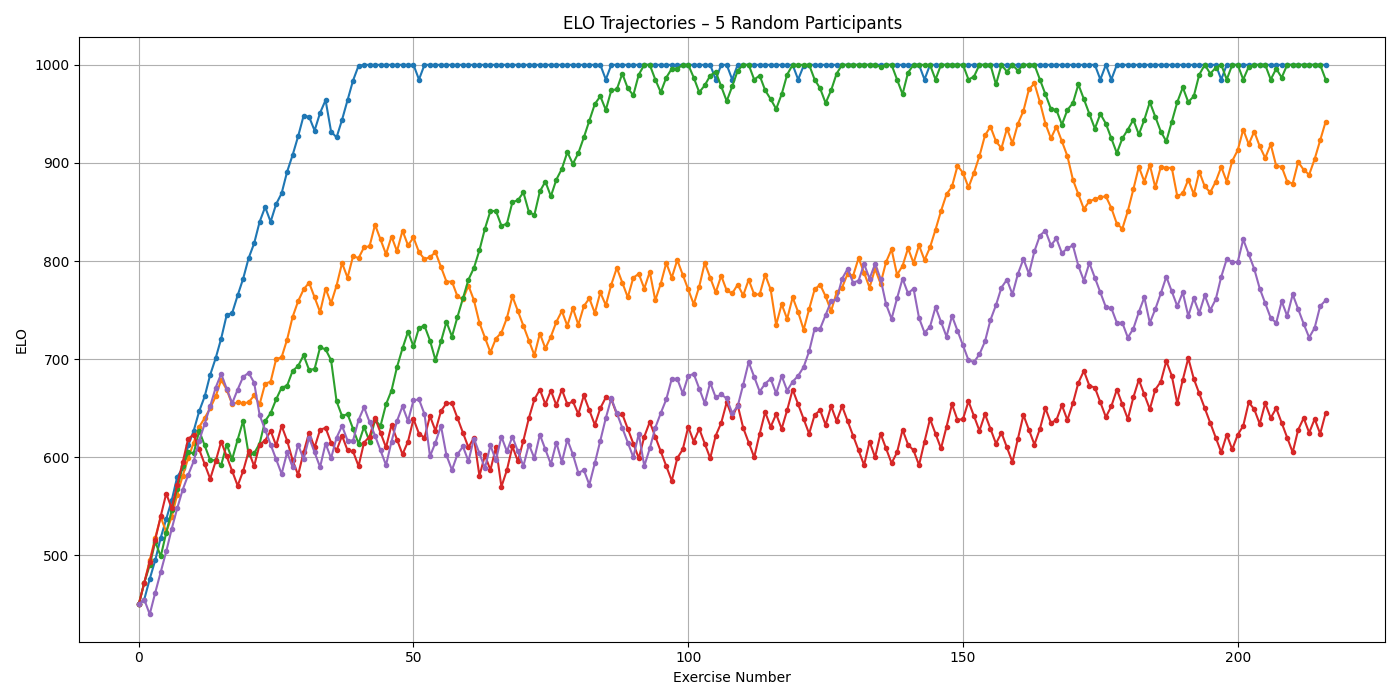
\includegraphics[width=\textwidth]{figures/sample_trajectories.png}
\caption{Elo rating trajectories of five randomly selected participants from the adaptive conditions. All participants started at a rating of 450. The trajectories illustrate how the system differentiates between children of different ability levels over the course of 216 exercises.}
\label{fig:elo-trajectories}
\end{figure}

\subsection{Final Elo distribution}
Figure~\ref{fig:elo-distribution} shows the distribution of final Elo scores across all participants in the adaptive conditions. The distribution spans from approximately 500 to 1000, with a main cluster around 600--700 and a second, distinct peak at the maximum rating of 1000. The main cluster sits in difficulty zone 4 (600--800), meaning these children were predominantly receiving difficult and medium exercises by the end of the training. The peak at 1000 represents children who reached the ceiling and stayed there. For these children, the exercise pool could no longer offer sufficient challenge, as all exercises were already drawn from the highest difficulty level.\\ \\
\begin{figure}[ht]
\centering
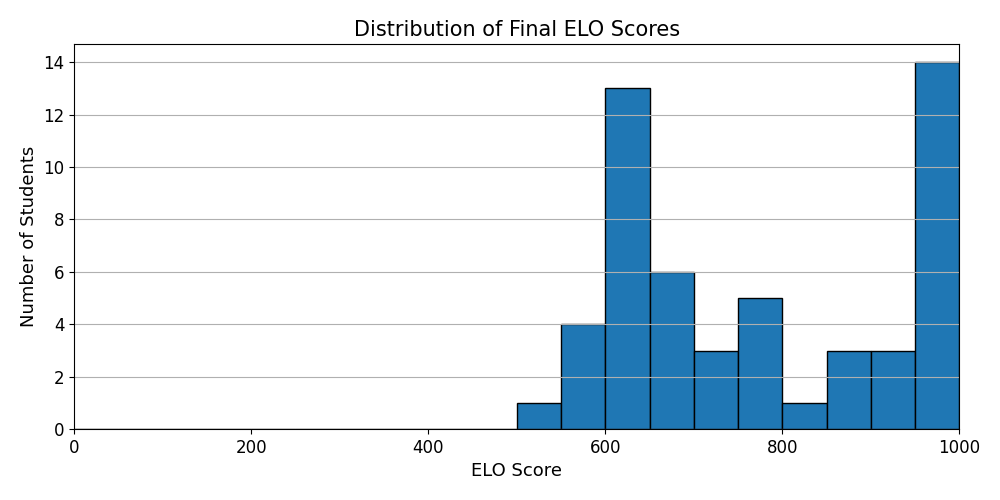
\includegraphics[width=0.8\textwidth]{figures/elo_distribution_histogram.png}
\caption{Distribution of final Elo scores across participants in the adaptive conditions. The main cluster around 600--700 corresponds to difficulty zone 4. The peak at 1000 represents children who reached the rating ceiling.}
\label{fig:elo-distribution}
\end{figure}

\subsection{Accuracy rates}
Figure~\ref{fig:accuracy-distribution} compares the distribution of per-student accuracy rates between the adaptive and non-adaptive conditions. The non-adaptive group achieved a mean accuracy of 76\% (\(\sigma = 0.16\)), which sits close to the 75\% target. The adaptive group achieved a lower mean accuracy of 68\% (\(\sigma = 0.14\)). The difference is expected: children in the adaptive conditions faced a higher average exercise difficulty (mean difficulty level of 2.54, compared to 2.00 in the non-adaptive conditions, where difficulty levels were balanced by design). The adaptive system pushed stronger children toward harder exercises, which increased the error rate.
However, the adaptive system did not converge on the intended 75\% accuracy target. The mean accuracy of 68\% indicates that the current parameter settings produce a difficulty level that is somewhat too challenging for the average participant. The most likely explanation is that the \(K\) parameter or the scoring function needs further tuning to achieve a closer match with the target. This is discussed further in Section \myworries{IN WHICH SETION IN DISCUSSIOn}.
\begin{figure}[ht]
\centering
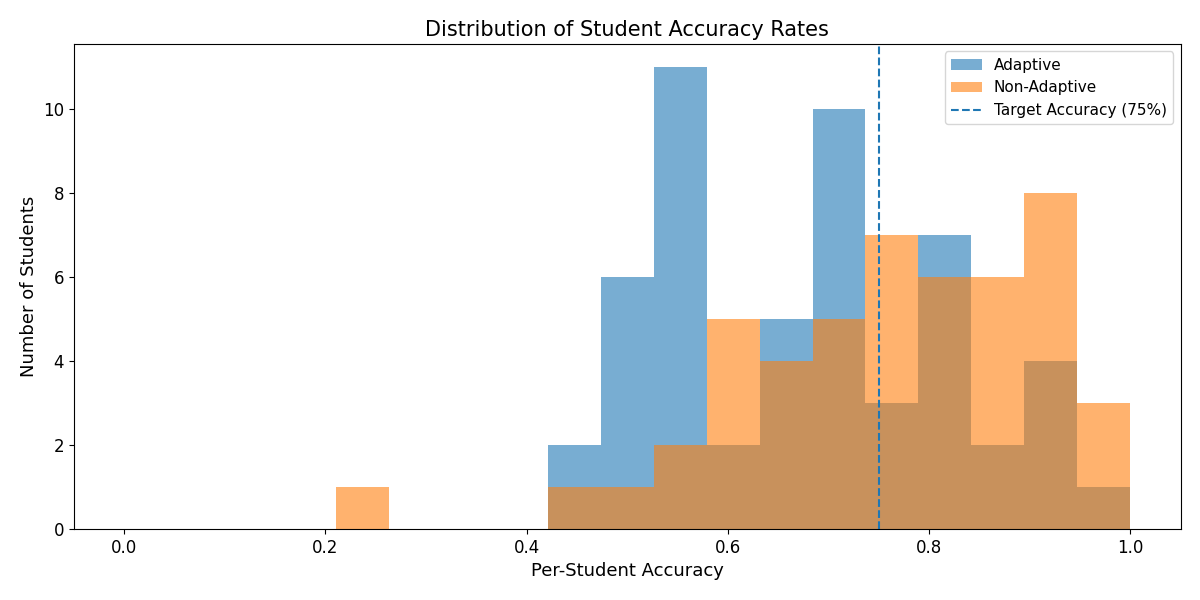
\includegraphics[width=\textwidth]{figures/accuracy_distribution_histogram.png}
\caption{Distribution of per-student accuracy rates for the adaptive and non-adaptive conditions. The dashed line marks the 75\% target accuracy. The adaptive group (mean 68\%) falls below the target, while the non-adaptive group (mean 77\%) lands close to it.}
\label{fig:accuracy-distribution}
\end{figure}

\subsection{Response times}
Figure~\ref{fig:response-time-distribution} shows the distribution of mean response times per student for both groups. The non-adaptive group shows a wide, relatively uniform spread across response times, ranging from around 6 to 14 seconds. This is consistent with the fact that these children received exercises from all three difficulty levels regardless of their ability: strong children solved easy exercises quickly while weaker children spent longer on the harder ones, producing a flat distribution. The adaptive group shows a different pattern, with a concentration toward longer response times (12--14 seconds). This is consistent with how the scoring function works: the system's equilibrium point occurs when a child answers correctly at approximately the time limit, which means the adaptive algorithm naturally pushes children toward exercises where they need close to the full time available.\\ \\
\begin{figure}[ht]
\centering
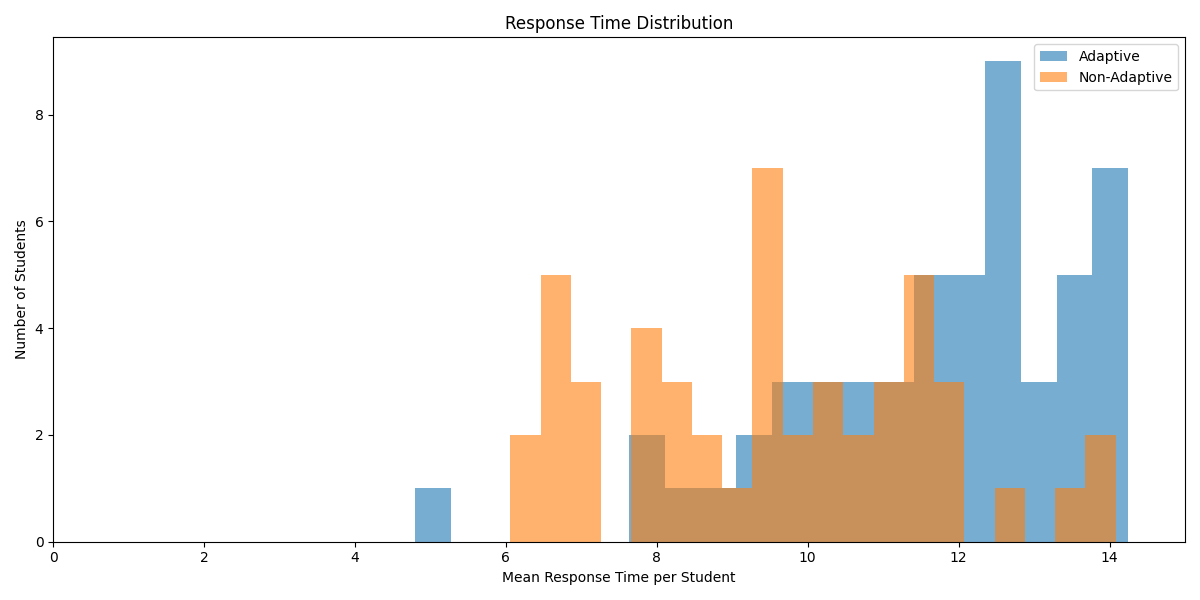
\includegraphics[width=\textwidth]{figures/response_time_distribution.png}
\caption{Distribution of mean response times per student for the adaptive and non-adaptive conditions. The adaptive group clusters toward longer response times, consistent with the scoring function pushing toward the time limit as an equilibrium point.}
\label{fig:response-time-distribution}
\end{figure}

\subsection{Qualitative observations}
The quantitative patterns are supported by observations made during the classroom sessions. In her feedback report, Eline T'joen noted that children in the non-adaptive conditions appeared to lose focus more quickly during exercises, while children in the adaptive conditions remained more consistently engaged. She also observed that the non-adaptive group showed visible signs of frustration or boredom more frequently, which aligns with the theoretical expectation from Section 3.1: when exercises do not match a child's level, the result is either anxiety (too hard) or disengagement (too easy). The adaptive system, despite not hitting its 75\% accuracy target precisely, appears to have produced a more engaging experience by keeping the challenge level closer to each child's ability.

\section{Engagement: coins and puzzles}
One of the central claims of this thesis is that gamification elements help keep children engaged across multiple sessions. The coin and puzzle system in RekenRangers provides a direct way to test this claim with behavioural data rather than self-report alone: if children actively spend their coins on puzzles, they are engaging with the gamification system, and if they complete puzzles, they are treating the animal rescue mission as a genuine subgoal.\\ \\
Table~\ref{tab:coin-summary} summarises the coin and puzzle data across all four conditions. The results are striking. Across the full sample of 107 participants, children spent on average 98.5\% of their earned coins on puzzle pieces. Out of 107 children, nobody spent less then 85\% of their coins. This pattern is consistent across all four conditions, regardless of whether the condition included metacognitive prompts or adaptive difficulty.\\ \\
\begin{table}[ht]
\centering
\small
\setlength{\tabcolsep}{6pt}

\begin{tabular}{@{}lcccccc@{}}
\toprule

Condition & \(n\) & Mean earned & Mean spent & Mean \% spent & Mean puzzles completed \\
\midrule
A & 27 & 671.0 & 659.8 & 98.3 & 2.5 \\
B & 27 & 685.2 & 673.7 & 98.2 & 2.6 \\
C & 27 & 610.4 & 601.9 & 98.6 & 2.0 \\
D & 26 & 620.7 & 613.5 & 98.8 & 2.0 \\
\bottomrule
\end{tabular}

\caption{Average coin earning, spending, and puzzle completion across the four experimental conditions. Children were free to spend or save their coins; no instructions or incentives to buy puzzle pieces were given beyond the narrative framing of the safari story.}
\label{tab:coin-summary}
\end{table}

\noindent It is worth emphasising that children were never instructed to spend their coins. The puzzle shop was available at the end of each training day, and children were told they could buy puzzle pieces if they wanted to, but there was no check or reward for doing so. The near-universal spending behaviour therefore reflects genuine voluntary engagement with the gamification system. The small number of unspent coins per child (on average between 0 and 25 coins depending on the condition) is largely explained by the fact that remaining coins were insufficient to purchase another puzzle piece at the prices available.\\ \\
The puzzle completion data adds a second layer to this picture. Across all conditions, 99\% of children completed at least one puzzle, and 47\% completed three or more over the four training days. The coin system was deliberately designed so that completing all six puzzles within 216 exercises was impossible, ensuring that there was always a next goal to work toward. Interestingly, the data also reveals different purchasing strategies: some children prioritised the cheaper puzzles to complete as many animals as possible, while others saved for more expensive puzzles and ended up with fewer completed puzzles despite having earned a similar number of coins. This variation in strategy suggests that children were not mindlessly clicking through the puzzle shop but were making deliberate choices about how to spend their resources.\\ \\
The difference in mean coins earned between the non-adaptive conditions (A and B, around 680 coins) and the adaptive conditions (C and D, around 615 coins) is expected: the adaptive system presents harder exercises to stronger children, which increases response times and reduces the coin bonus for speed. This does not appear to have affected engagement, as the spending percentages in all four conditions were in fact highly similar.\\ \\

\section{Questionnaire results}

\section{Researcher feedback}
